\section{Framework}

The framework is divided in two: The physical world and the game world. All things only existing in the physical world operates on this side, and everything diegetic to the game world, i.e. what can be seen, heard, felt, tasted, smelled, touched, etc. by an agent in the game world operates on the game world side. All information transferred between these divisions is send and/or received through the augmented information of the real world.
Furthermore, the framework is divided horizontally in feedforward on top and feedback at the bottom. This is done to avoid confusion that may arise when trying to discern if a coupling is through feedforward or feedback, which has arisen in other adaptations of the Frogger Framework \cite{tangifrog}.

\begin{figure}
  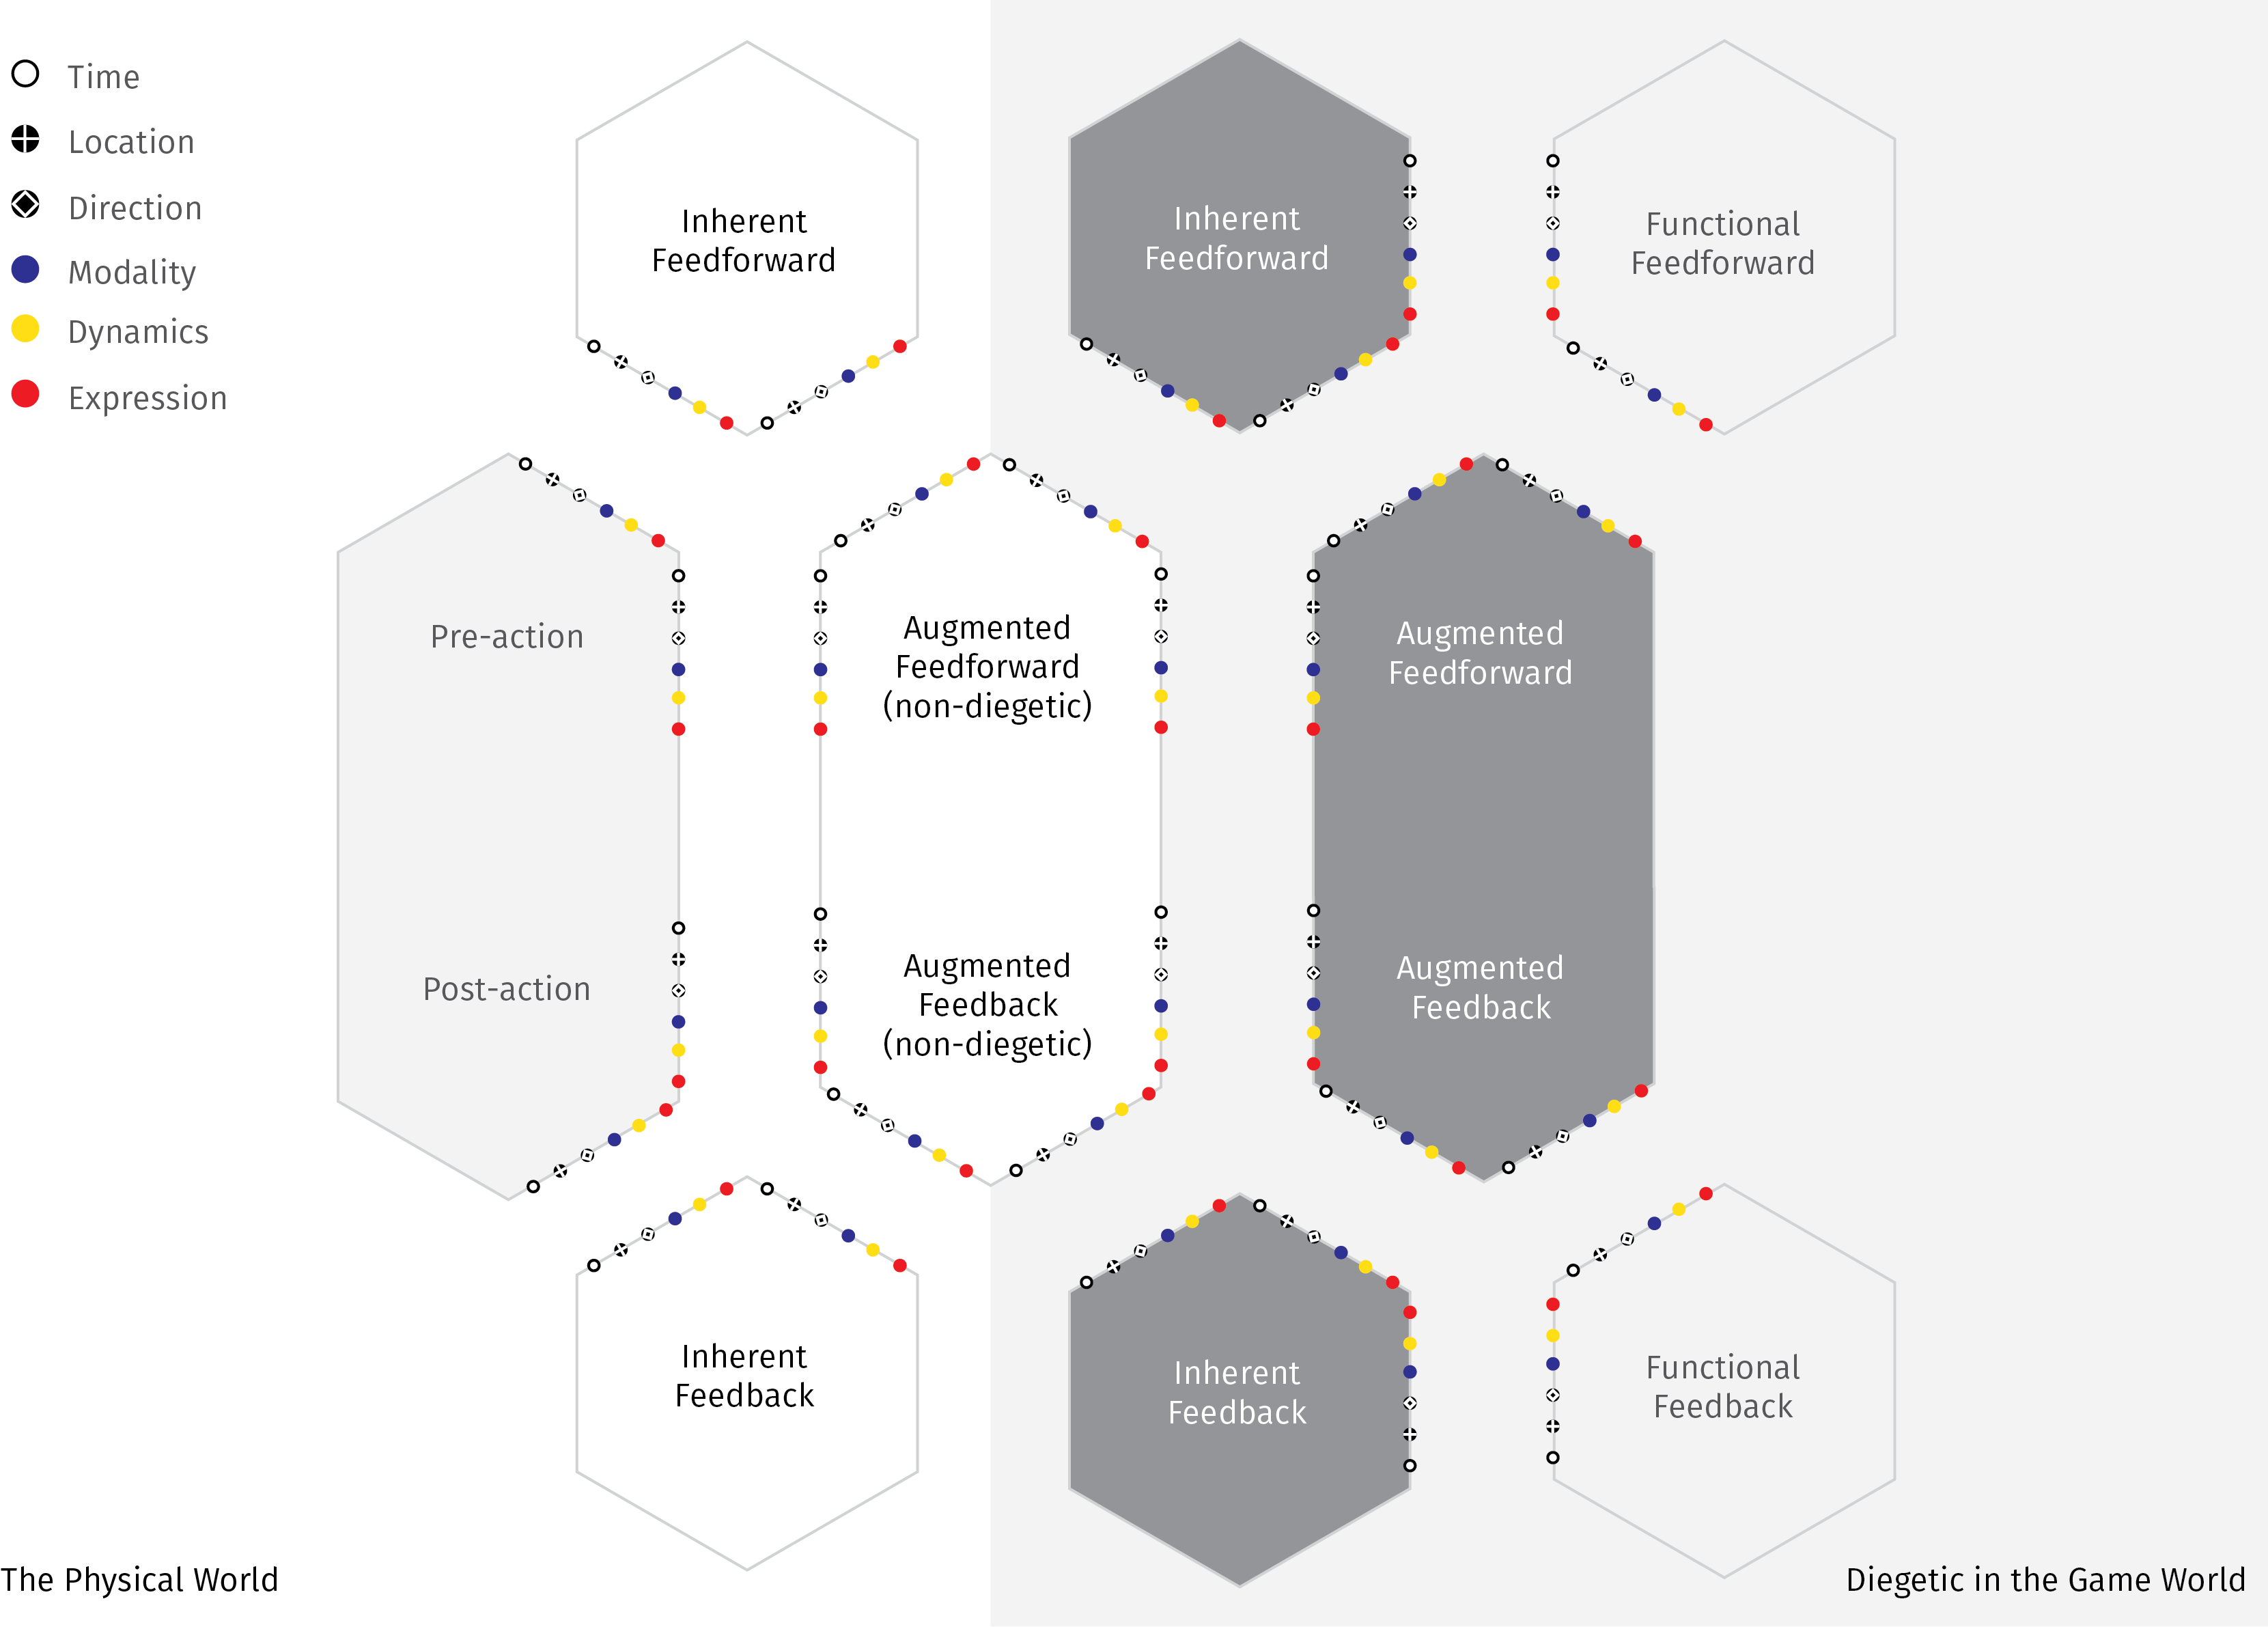
\includegraphics[width=\textwidth]{Framework}
  \caption{The Framework}
  \label{framework}
\end{figure}

\subsection{Physical World}
\cite{norman} \cite{frogger} \cite{dourish}

\subsection{Diegetic to the Game World}
Totten, Rollings, Vella

\subsubsection{Inherent Information in a Game World}
Everything diegetic to the game world that uses inherent information (hills or tar that make you walk slower, elastics, wheels). Is highly tied to the conceptual model of the player, i.e. how does physics work.

\subsubsection{Augmented Information in a Game World}
Everything diegetic to the game world that uses augmented information (stop signs, buttons, signifiers). It is not a HUD since that does not exist in the game world. A HUD is augmented information in the physical world.

\subsection{Scope}
The framework cannot be used to analyse a game as a whole, but works better the smaller the focus. It can for example be used to analyse how a mechanic is conveyed EXAMPLE, how a mechanic is used, how a challenge is perceived, how a challenge is solved

\subsection{Limitations}
Complexity of computer systems: "The consequence, then, is that there are very many different levels of description that could be used to describe my activity at any given moment. Some, perhaps, are ready-to-hand and some present-at-hand at the same time; my orientation toward them each will change. For instance, sometimes as I move the mouse, the mouse itself is the focus of my attention; some-times I am directed instead toward the cursor that it controls on the screen; at other times, I am directed toward the button I want to push, the e-mail message I want to send, or the lunch engagement I am trying to make" \cite[p. 140]{dourish}. Therefore, it is difficult to discern complex systems. Framework should be considered a talking point; more like a sketch than a drawing.
